\chapter{Desarrollo}

\section{Hardware}

El hardware se diseña por medio del software Proteus ...

\section{Firmware}

El firmware se desarrolla sobre el framework o SDK oficial de Espressif Systems, ESP-IDF el cual posee una documentación \cite{ES}, la cuál es muy útil a la hora de utilizar las diferentes APIs que este posee. Este firmware incluye un kernel de tiempo real llamado FreeRTOS, el cual da soporte al manejo de los diferentes recursos del sistema. Como es un RTOS, las funciones se definen mediante las tareas, entonces para cada funcionalidad de la tarjeta o grupo de funcionalidades se desarrolla una o varias tareas para que realicen las acciones adecuadas, por ejemplo, en cuanto a los sensores cada uno tiene una tarea para su lectura, gestión de estos datos, así, como también en cuanto a las diferentes salidas de la tarjeta se han agrupado en las cargas que solo son de encendido/apagado y las de control, creando diferentes tareas para esta gestión.\\

Sobre el firmware se desarrollan los siguientes temas:

\paragraph{Tareas:}

como se menciona anteriormente, estas cumplen las funciones principales en cuanto a toda la gestión de los diferentes periféricos y funcionalidades de la tarjeta, así que se desarrollan diferentes tareas para la lectura y escritura en los puertos de la tarjeta.

\paragraph{GPIO:}

el ESP-WROOM-32 posee diferentes GPIO, los cuales se usan para leer o escribir señales digitales, en cuanto a los sensores se pueden enviar señales para iniciar su lectura o simplemente tener el pin en modo entrada y leerlo cada cierto intervalo de tiempo para generar los datos de lectura, o en modo salida para el control de los diferentes dispositivos que se han desarrollado en el hardware.

\paragraph{ADC,DAC:}

los ADC se usan para leer los datos de algunos sensores que proporcionan datos analógicos, por este motivo se hace la conversión de la señal analógica a un valor digital dentro de la tarjeta, para luego identificar el valor de la lectura del sensor. Los DAC se usan para realizar la operación contraria, teniendo valores digitales convertirlos a un valor analógico por ejemplo para generar audios o diferentes señales a partir del software.

\paragraph{Consola:}

para realizar diferentes pruebas directamente desde la tarjeta, se usa la opción de la consola que se comunica por medio del puerto serie, para esto se crean las funciones y los comandos que estaran disponibles. Algunos comandos disponibles son \textit{http}, para realizar las peticiones http manualmente y observar su respuesta, pin para realizar la prueba de un pin digital como entrada o salida, \textit{help} para observar la lista de comandos, entre otros.

\paragraph{HTTP Request:}

las peticiones HTTP son indispensables en estas aplicaciones del campo IOT, por este motivo en el desarrollo del firmware se usan las librerias pertinentes para realizar peticiones y además leer las respuestas de estas desde el servidor, ya que este es el medio de comunicación tarjeta-servidor.

\paragraph{Hora de Red:}

se obtiene la hora mediante el protocolo simple de tiempo de red (SNTP), este resulta de gran utilidad para la sincronización de los relojes de los sistemas informáticos.

\paragraph{Timers:}

la tarjeta posee dos grupos de timers, que cuenta cada uno con dos timers, un timer lo usa el sistema operativo, otro es configurado para realizar el control de potencia AC por ángulo de fase, para tener la sincronía necesaria con la señal de la red eléctrica.

\paragraph{I2C:}

el protocolo I2C se activa por medio de la instalación del driver en algún par de pines GPIO disponibles en la tarjeta. Se configura e inicia y posteriormente se crea una tarea la cuál se encarga de solicitar y leer los datos de los diferentes sensores conectados a este.

\paragraph{PWM:}

se ha mencionado anteriormente que para controlar las cargas DC se usa una salida PWM, el esp32 proporciona esta funcionalidad en algunos de sus pines, para su uso se configura y asignan los valores de funcionamiento.

\paragraph{Interrupciones:}

las interrupciones se usan para no gastar recursos en un monitoreo constante de las entradas, solo cuando exista un cambio de nivel en la entrada el dispositivo desencadena una serie de instrucciones relacionas al tipo de interrupción y a diferentes funciones creadas para esta, la interrupción se usa por medio de los diferentes pines propuestos para esto en el hardware.

\section{Software}

En esta sección se desarrolla una aplicación web, la cual se encarga de hacer la gestión entre el usuario y la tarjeta. De este modo, se usa un patron de arquitectura Modelo-Vista-Controlador (MVC) para esta aplicación, este modelo es realmente util ya que separa la lógica de negocio de la interfaz de usuario, incrementando la reutilización y flexibilidad y además la escalabilidad de ambos aspectos por separado, dicho esto la aplicación cuenta con diferentes modelos, controladores y vistas. La función de cada parte de esta arquitectura se puede observar en la figura \ref{fig:mvc}.\\

%https://www.fdi.ucm.es/profesor/jpavon/poo/2.14.MVC.pdf
%https://si.ua.es/es/documentacion/asp-net-mvc-3/1-dia/modelo-vista-controlador-mvc.html

\begin{figure}
	\centering
	\caption{Modelo-Vista-Controlador}
	\label{fig:mvc}
	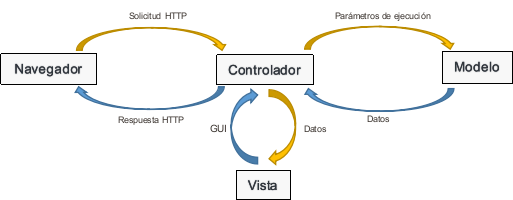
\includegraphics[width=0.7\linewidth]{Imagenes/MVC}
\end{figure}


El flujo es el siguiente, primero el usuario realiza alguna acción en la interfaz (por ejemplo, presiona un boton, un enlace, etc), luego el controlador recibe (por parte de los objetos de la interfaz-vista) la notificación de la acción solicitada por el usuario. El controlador gestiona el evento que llega. Luego el controlador accede al modelo, actualizándolo, posiblemente modificándolo de forma adecuada a la acción solicitada por el usuario (por ejemplo, el controlador actualiza los datos del perfil del usuario) y después la interfaz de usuario espera nuevas interacciones del usuario, comenzando el ciclo nuevamente.\\

Este patron de diseño se usa en la programación orientada a objetos, por lo tanto se realiza la aplicación en el lenguaje de programación PHP, ya que es realmente util para realizar la gestión de peticiones y envíos de formularios en dicha aplicación, además de que es importante también la gestión de las bases de datos de la aplicación, por este motivo se utiliza un framework basado en este lenguaje y esta arquitectura, el cual realiza diferentes trabajos en cuanto a la parte de la arquitectura, para gestionar las diferentes partes de la aplicación, en este caso se usa el framework Laravel el cual como se menciona anteriormente esta orientado a facilitar las tareas comunes de la mayoría de proyectos web, que utilizan HTML5 y PHP.\\

Además, con este framework se hace uso de un ORM (Mapeo Objeto-Relacional) llamado Eloquent. Esta es una forma de mapear los datos que se encuentran en la base de datos a objetos de PHP y viceversa, esto facilita el uso de diferentes gestores de bases de datos como MySQL, SQLite, entre otras, ya que todas las consultas estan en PHP y el ORM ya se encarga del mapeo a los comandos SQL como se observa en la figura \ref{fig:orm}. Eloquent usa los modelos para enviar y recibir la información de la base de datos.

\begin{figure}[H]
	\centering
	\caption{ORM}
	\label{fig:orm}
	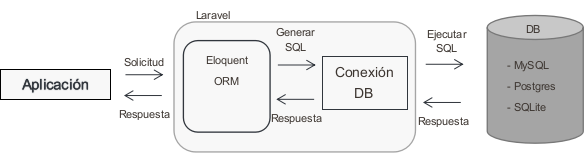
\includegraphics[width=0.7\linewidth]{Imagenes/ORM}
\end{figure}


%https://richos.gitbooks.io/laravel-5/capitulos/chapter7.html
%http://www.diva-portal.org/smash/get/diva2:1014983/FULLTEXT02